\documentclass[]{article}

\usepackage[utf8]{inputenc}
\usepackage{amsmath}
\usepackage{amssymb}
\usepackage{amsthm}
\usepackage{amsfonts}
\usepackage{graphicx}
\usepackage{capt-of}
\usepackage{listings}
\usepackage{siunitx}
\usepackage[section]{placeins}
\usepackage{multicol}
\usepackage[a4paper, portrait, margin=1in]{geometry}
\usepackage{float}
\usepackage{xcolor}

% Solarized colour scheme for listings
\definecolor{solarized@base03}{HTML}{002B36}
\definecolor{solarized@base02}{HTML}{073642}
\definecolor{solarized@base01}{HTML}{586e75}
\definecolor{solarized@base00}{HTML}{657b83}
\definecolor{solarized@base0}{HTML}{839496}
\definecolor{solarized@base1}{HTML}{93a1a1}
\definecolor{solarized@base2}{HTML}{EEE8D5}
\definecolor{solarized@base3}{HTML}{FDF6E3}
\definecolor{solarized@yellow}{HTML}{B58900}
\definecolor{solarized@orange}{HTML}{CB4B16}
\definecolor{solarized@red}{HTML}{DC322F}
\definecolor{solarized@magenta}{HTML}{D33682}
\definecolor{solarized@violet}{HTML}{6C71C4}
\definecolor{solarized@blue}{HTML}{268BD2}
\definecolor{solarized@cyan}{HTML}{2AA198}
\definecolor{solarized@green}{HTML}{859900}

\lstset{language=C++,
        basicstyle=\footnotesize\ttfamily,
        numbers=left,
        numberstyle=\footnotesize,
        tabsize=2,
        breaklines=true,
        escapeinside={@}{@},
        numberstyle=\tiny\color{solarized@base01},
        keywordstyle=\color{solarized@green},
        stringstyle=\color{solarized@cyan}\ttfamily,
        identifierstyle=\color{solarized@blue},
        commentstyle=\color{solarized@base01},
        emphstyle=\color{solarized@red},
        frame=single,
        rulecolor=\color{solarized@base2},
        rulesepcolor=\color{solarized@base2},
        showstringspaces=false
}



% Oppgavenummerering %
\renewcommand\thesection{Task \arabic{section}}
\renewcommand\thesubsection{\alph{subsection})}
\renewcommand\thesubsubsection{\roman{subsubsection})}

% Bevis
\newcommand\TombStone{\rule{.5em}{.5em}}
\renewcommand\qedsymbol{\TombStone}

\title{\Huge{Assignment 2} \\ \Large{TDT4195 – Visual Computing Fundamentals}}
\author{Sigurd Totland | MTTK}

\begin{document}
\maketitle
\begin{multicols}{2}
\section{Repetition}
\subsection{}
We create two VBOs. One for vertices and one for the color of said vertices.

\subsection{}
To show off our vertex coloring, we create six triangles that are for now non-overlapping. We define our triangles and colors as shown in listing \ref{lst:6_tris_1}. The index set is simply generated and contains values like $1,2,3,\dots$, i.e. our triangle vertices are specified in the order that they are rendered, and are thus specified in such an order that their triangles wind correctly. We pass the color values through the vertex shader, and use them in the fragment shader. The result is shown in figure \ref{fig:6_tris_1} below.
\begin{figure}[H]
\centering

\includegraphics[width=\columnwidth]{6_color_tris.png}
\caption{Six gradient-colored triangles.}
\label{fig:6_tris_1}
\end{figure}

\section{Blending and Depth}
\subsection{}
We turn on alpha blending and create three transparent, overlapping triangles overlapping at $z = 0.0$, $z=0.1$ and $z=0.2$ with different colors. We make sure that they are draw back-to-front. The result when using blending function \texttt{GL\_ONE\_MINUS\_SOURCE\_ALPHA} is shown in figure \ref{fig:overlap}.
\begin{figure}[H]
\centering

\includegraphics[width=0.5\columnwidth]{overlap.png}
\caption{Overlapping triangles.}
\label{fig:overlap}
\end{figure}
\subsection{}
\subsubsection{}
Changing the front triangle to green, shown in figure \ref{fig:overlap2} makes the blended colors different.
\begin{figure}[H]
\centering

\includegraphics[width=0.5\columnwidth]{overlap2.png}
\caption{Overlapping triangles, green in front.}
\label{fig:overlap2}
\end{figure}
This becomes especially clear if we look at the center triangles separately. These are shown in figure \ref{fig:tris_centers}.
\begin{figure}[H]
\centering

\includegraphics[width=0.5\columnwidth]{tris_centers.png}
\caption{Overlapping triangle centers.}
\label{fig:tris_centers}
\end{figure}
Clearly, the one with the green triangle in front (left triangle) is much more green than the other. We can analyze the resulting colors. As can be seen in figure \ref{fig:colors}, the triangles contain equal amounts of red, but the green and blue colors switch place, exactly as expected.
\begin{figure}[H]
\centering
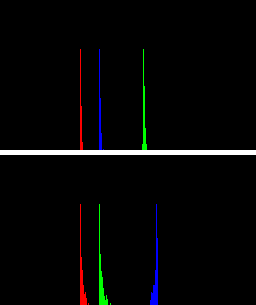
\includegraphics[width=0.5\columnwidth]{colors.png}
\caption{Color intensities. Top: green tri in front. Bottom: blue tri in front.}
\label{fig:colors}
\end{figure}

\subsubsection{}
We now try to exchange the order triangle order through the z-coordinate. Placing the front triangle (the blue triangle, which we recall is \textit{drawn last} of the three) inbetween the red and the green, we obtain the (perhaps unexpected) result in figure \ref{fig:overlap3}
\begin{figure}[H]
\centering

\includegraphics[width=0.5\columnwidth]{overlap3.png}
\caption{Depth and draw order mismatched.}
\label{fig:overlap3}
\end{figure}
This result can be understood by understanding how we emulate transparency in OpenGL and how it relates to the z-buffer. Before painting the fragments of any triangle, transparent or not, we look at at the index buffer for the current fragment. When using \texttt{GL\_LESS}, if the buffer contains a smaller value than the z-coordinate of the current fragment, it means that some other shape has already been drawn in front and the fragment is hence not painted. In our case, the green triangle is in front of the blue, so upon drawing the blue (which happens after the green) OpenGL does not paint any of the fragments that overlap with the green. For an example of the intended behaviour, we can look at the red and green triangles. The red is really behind the green, but it gets drawn first. So when painting it, every fragment passes the depth test, and are subsequently painted. Afterwards, when the green triangle gets drawn, it (also passing the depth test entirely) gets drawn fully, but because we have enabled alpha blending, the colors drawn get calculated from the blending function. To summarize, the three triangle draws that OpenGL does is shown (from left to right) in figure \ref{fig:steps}.
\begin{figure}[H]
\centering

\includegraphics[width=\columnwidth]{steps.png}
\caption{Draw steps.}
\label{fig:steps}
\end{figure}

\end{multicols}
\appendix
\section{C++ snippets}
\begin{lstlisting}[language={C++}, caption={Vertices for 6 triangles}, label={lst:6_tris_1}]
std::vector<float> triangleCoords {
   -0.4, 0.05, 0.0,
    -0.4, 0.5, 0.0,
    -0.9, 0.05, 0.0,

    0.8, 0.05, 0.0,
    0.8, 0.5, 0.0,
    0.3, 0.05, 0.0,

    0.2, 0.05, 0.0,
    0.2, 0.5, 0.0,
    -0.3, 0.05, 0.0,

    -0.4, -0.5, 0.0,
    -0.4, -0.05, 0.0,
    -0.9, -0.05, 0.0,

    0.8, -0.5, 0.0,
    0.8, -0.05, 0.0,
    0.3, -0.05, 0.0,

    0.2, -0.5, 0.0,
    0.2, -0.05, 0.0,
    -0.3, -0.05, 0.0,
}


std::vector<float> triangleColors {
    0.1, 0.1, 0.1, 0.7, // Black
    0.9, 0.1, 0.3, 0.7, // Red
    0.1, 0.1, 0.1, 0.7, // Black

    0.1, 0.1, 0.1, 0.7, // Black
    0.1, 0.8, 0.0, 0.7, // Green
    0.1, 0.1, 0.1, 0.7, // Black

    0.1, 0.1, 0.1, 0.7, // Black
    0.1, 0.1, 0.9, 0.7, // Blue
    0.1, 0.1, 0.1, 0.7, // Black

    0.9, 0.1, 0.9, 0.7, // Magenta
    0.1, 0.1, 0.1, 0.7, // Black
    0.1, 0.1, 0.1, 0.7, // Black

    0.7, 0.8, 0.0, 0.7, // Yellow
    0.1, 0.1, 0.1, 0.7, // Black
    0.1, 0.1, 0.1, 0.7, // Black

    0.1, 0.8, 0.8, 0.7, // Cyan
    0.1, 0.1, 0.1, 0.7, // Black
    0.1, 0.1, 0.1, 0.7, // Black
};

\end{lstlisting}

\end{document}

